\section{Eksisterende systemer}
Bla bla bla introduktion.

\subsection{Ginger.io}
Ginger.io er en app til iPhone og Android, beregnet til at assistere patienter med diverse psykiskse lidelser.\cite{ginger_dot_io}\cite{gingerio_mit}\cite{gingerio_dailymail}


App'en er lavet til at assistere i behandlingen for følgende lidelser: depression, angst, bipolær affektiv lidelse og skizofreni.

Efter at app'en er installeret, vil den indsamle data, hvilket kan sige noget om mobil-brugerens sindsmæssige tilstand.
Der bliver overordnet set indsamlet to typer data; aktiv og passiv.
Den aktive data er forespørgsler fra app'en, hvor mobil-brugeren selv skal svare.
Den passive data vil blive indsamlet i baggrunden, og består af interaktions- og lokations-data, hvor interaktions-data er mobil-brugerens opkald- og SMS-vaner og lokations-data er opfanget via GPS og accelerometer, for at sige noget om hvor og hvordan mobil-brugeren bevæger og opholder sig.

For at komme i gang med app'en, skal brugeren indtaste relevant information, såsom diagnoser, behandlingsforløb og behandler.
Ud fra disse informationer vil app'en tilpasse forespørgslerne brugt til indsamling af aktiv data.
Derudover vil den passive data der indsamles i de første dage bruges til at angive brugerens normal-tilstand.
Herefter vil brugeren modtage notifikationer om ændret tilstand i social eller fysisk aktivitet, og i værste tilfælde vil behandler eller anden angivet kontaktperson blive notificeret.

Brugere af Ginger.io skal være forbundet gennem en behandler, og denne behandler vil til enhver tid have adgang til alle brugerens informationer.
Den overordnede idé er at Ginger.io skal assistere behandlingsprocessen, ved at give en indikator på brugerens tilstand mellem klinikbesøg (se \cref{eksisterende_systemer:ginger_io_graf}).

\begin{figure}[h]
\centering
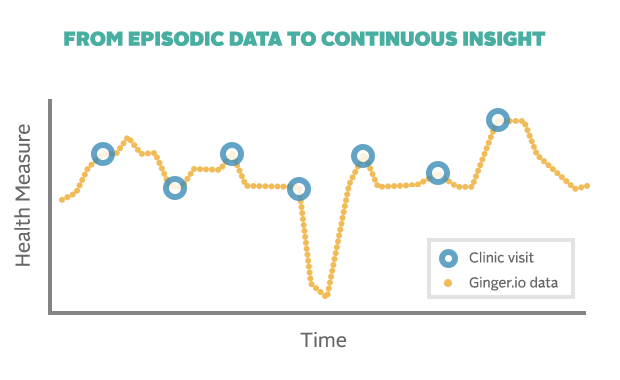
\includegraphics[width=.75\textwidth]{ginger_io_graph}
\caption{Figur fra https://ginger.io/for-providers/}
\label{eksisterende_systemer:ginger_io_graf}
\end{figure}

\subsubsection*{Problemer}
Som det ser ud nu, er Ginger.io kun tilgængeligt i USA, og kun ved tilmeldte behandlere.
Derudover fungere interaktions-data-indsamlingen kun på Android, hvilket betyder at iPhone app'en kun indsamler lokation-data og den aktive data.

\subsection{Fitness Trackere}
Der findes adskillige apps og større systemer til at styre ens fysiske aktivitet og velvære.
Heriblandt;
\begin{itemize}
\item Apple Health\cite{apple_health}
\item Google Fit\cite{google_fit}
\item Microsoft Health\cite{ms_health} / HealthVault\cite{ms_health_vault}
\item S Health\cite{s_health}
\end{itemize}

Ens for disse fitness trackere, i modsætning til enkelte apps, er at de samler informationer, fra et væld af forbundne enheder, ét sted.
Ydermere er de designet til at kunne indstilles til bestemte mål, og kan derved fortælle løbende om hvordan det går med at opnå disse mål.
